%%%%%%%%%%%%%%%%%%%%%%%%%%%%%%%%%%%%%%%%%
% Lachaise Assignment
% LaTeX Template
% Version 1.0 (26/6/2018)
%
% This template originates from:
% http://www.LaTeXTemplates.com
%
% Authors:
% Marion Lachaise & François Févotte
% Vel (vel@LaTeXTemplates.com)
%
% License:
% CC BY-NC-SA 3.0 (http://creativecommons.org/licenses/by-nc-sa/3.0/)
% 
%%%%%%%%%%%%%%%%%%%%%%%%%%%%%%%%%%%%%%%%%

%----------------------------------------------------------------------------------------
%	PACKAGES AND OTHER DOCUMENT CONFIGURATIONS
%----------------------------------------------------------------------------------------

\documentclass{article}

%%%%%%%%%%%%%%%%%%%%%%%%%%%%%%%%%%%%%%%%%
% Lachaise Assignment
% Structure Specification File
% Version 1.0 (26/6/2018)
%
% This template originates from:
% http://www.LaTeXTemplates.com
%
% Authors:
% Marion Lachaise & François Févotte
% Vel (vel@LaTeXTemplates.com)
%
% License:
% CC BY-NC-SA 3.0 (http://creativecommons.org/licenses/by-nc-sa/3.0/)
% 
%%%%%%%%%%%%%%%%%%%%%%%%%%%%%%%%%%%%%%%%%

%----------------------------------------------------------------------------------------
%	PACKAGES AND OTHER DOCUMENT CONFIGURATIONS
%----------------------------------------------------------------------------------------

\usepackage{amsmath,amsfonts,stmaryrd,amssymb} % Math packages

\usepackage{graphicx}

\usepackage{dblfloatfix}

\usepackage{hyperref}

\usepackage[makeroom]{cancel}

\usepackage{enumerate} % Custom item numbers for enumerations

\usepackage[ruled]{algorithm2e} % Algorithms

\usepackage[framemethod=tikz]{mdframed} % Allows defining custom boxed/framed environments

\usepackage{listings} % File listings, with syntax highlighting
\lstset{
	basicstyle=\ttfamily, % Typeset listings in monospace font
}

%----------------------------------------------------------------------------------------
%	DOCUMENT MARGINS
%----------------------------------------------------------------------------------------

\usepackage{geometry} % Required for adjusting page dimensions and margins

\geometry{
	paper=a4paper, % Paper size, change to letterpaper for US letter size
	top=2.5cm, % Top margin
	bottom=3cm, % Bottom margin
	left=2.5cm, % Left margin
	right=2.5cm, % Right margin
	headheight=14pt, % Header height
	footskip=1.5cm, % Space from the bottom margin to the baseline of the footer
	headsep=1.2cm, % Space from the top margin to the baseline of the header
	%showframe, % Uncomment to show how the type block is set on the page
}

%----------------------------------------------------------------------------------------
%	FONTS
%----------------------------------------------------------------------------------------

\usepackage[utf8]{inputenc} % Required for inputting international characters
\usepackage[T1]{fontenc} % Output font encoding for international characters

\usepackage{XCharter} % Use the XCharter fonts

%----------------------------------------------------------------------------------------
%	COMMAND LINE ENVIRONMENT
%----------------------------------------------------------------------------------------

% Usage:
% \begin{commandline}
%	\begin{verbatim}
%		$ ls
%		
%		Applications	Desktop	...
%	\end{verbatim}
% \end{commandline}

\mdfdefinestyle{commandline}{
	leftmargin=10pt,
	rightmargin=10pt,
	innerleftmargin=15pt,
	middlelinecolor=black!50!white,
	middlelinewidth=2pt,
	frametitlerule=false,
	backgroundcolor=black!5!white,
	frametitle={Command Line},
	frametitlefont={\normalfont\sffamily\color{white}\hspace{-1em}},
	frametitlebackgroundcolor=black!50!white,
	nobreak,
}

% Define a custom environment for command-line snapshots
\newenvironment{commandline}{
	\medskip
	\begin{mdframed}[style=commandline]
}{
	\end{mdframed}
	\medskip
}

%----------------------------------------------------------------------------------------
%	FILE CONTENTS ENVIRONMENT
%----------------------------------------------------------------------------------------

% Usage:
% \begin{file}[optional filename, defaults to "File"]
%	File contents, for example, with a listings environment
% \end{file}

\mdfdefinestyle{file}{
	innertopmargin=1.6\baselineskip,
	innerbottommargin=0.8\baselineskip,
	topline=false, bottomline=false,
	leftline=false, rightline=false,
	leftmargin=2cm,
	rightmargin=2cm,
	singleextra={%
		\draw[fill=black!10!white](P)++(0,-1.2em)rectangle(P-|O);
		\node[anchor=north west]
		at(P-|O){\ttfamily\mdfilename};
		%
		\def\l{3em}
		\draw(O-|P)++(-\l,0)--++(\l,\l)--(P)--(P-|O)--(O)--cycle;
		\draw(O-|P)++(-\l,0)--++(0,\l)--++(\l,0);
	},
	nobreak,
}

% Define a custom environment for file contents
\newenvironment{file}[1][File]{ % Set the default filename to "File"
	\medskip
	\newcommand{\mdfilename}{#1}
	\begin{mdframed}[style=file]
}{
	\end{mdframed}
	\medskip
}

%----------------------------------------------------------------------------------------
%	NUMBERED QUESTIONS ENVIRONMENT
%----------------------------------------------------------------------------------------

% Usage:
% \begin{question}[optional title]
%	Question contents
% \end{question}

\mdfdefinestyle{question}{
	innertopmargin=1.2\baselineskip,
	innerbottommargin=0.8\baselineskip,
	roundcorner=5pt,
	nobreak,
	singleextra={%
		\draw(P-|O)node[xshift=1em,anchor=west,fill=white,draw,rounded corners=5pt]{%
		%\theQuestion
		\questionTitle};
	},
}

\newcounter{Question} % Stores the current question number that gets iterated with each new question

% Define a custom environment for numbered questions
\newenvironment{question}[1][\unskip]{
	\bigskip
	%\stepcounter{Question}
	\newcommand{\questionTitle}{~#1}
	\begin{mdframed}[style=question]
}{
	\end{mdframed}
	\medskip
}

%----------------------------------------------------------------------------------------
%	WARNING TEXT ENVIRONMENT
%----------------------------------------------------------------------------------------

% Usage:
% \begin{warn}[optional title, defaults to "Warning:"]
%	Contents
% \end{warn}

\mdfdefinestyle{warning}{
	topline=false, bottomline=false,
	leftline=false, rightline=false,
	nobreak,
	singleextra={%
		\draw(P-|O)++(-0.5em,0)node(tmp1){};
		\draw(P-|O)++(0.5em,0)node(tmp2){};
		\fill[black,rotate around={45:(P-|O)}](tmp1)rectangle(tmp2);
		\node at(P-|O){\color{white}\scriptsize\bf !};
		\draw[very thick](P-|O)++(0,-1em)--(O);%--(O-|P);
	}
}

% Define a custom environment for warning text
\newenvironment{warn}[1][Warning:]{ % Set the default warning to "Warning:"
	\medskip
	\begin{mdframed}[style=warning]
		\noindent{\textbf{#1}}
}{
	\end{mdframed}
}

%----------------------------------------------------------------------------------------
%	INFORMATION ENVIRONMENT
%----------------------------------------------------------------------------------------

% Usage:
% \begin{info}[optional title, defaults to "Info:"]
% 	contents
% 	\end{info}

\mdfdefinestyle{info}{%
	topline=false, bottomline=false,
	leftline=false, rightline=false,
	nobreak,
	singleextra={%
		\fill[black](P-|O)circle[radius=0.4em];
		\node at(P-|O){\color{white}\scriptsize\bf !};
		\draw[very thick](P-|O)++(0,-0.8em)--(O);%--(O-|P);
	}
}

% Define a custom environment for information
\newenvironment{info}[1][Info:]{ % Set the default title to "Info:"
	\medskip
	\begin{mdframed}[style=info]
		\noindent{\textbf{#1}}
}{
	\end{mdframed}
}
 % Include the file specifying the document structure and custom commands

%----------------------------------------------------------------------------------------
%	ASSIGNMENT INFORMATION
%----------------------------------------------------------------------------------------

\title{SerDes analog circuits description} % Title of the assignment

\author{Fávero Santos\\ \texttt{favero.santos@gmail.com}} % Author name and email address

\date{Revision 00 of \today} % University, school and/or department name(s) and a date

%----------------------------------------------------------------------------------------

\begin{document}

\maketitle % Print the title

%----------------------------------------------------------------------------------------
%	INTRODUCTION
%----------------------------------------------------------------------------------------

\section*{Introduction}

The netlists presented in this article can be seen as circuits if a netlist-to-schematic conversor (such as NetlistViewer - https://sourceforge.net/p/netlistviewer/wiki/Home/) is employed.

\begin{info}[\itshape Employed notation:] % Information block
	\begin{enumerate}[i]
		\item A DC only voltage/current is represented by an italic uppercase letter(s) followed by italic uppercase subscript letter(s).
		\subitem A DC voltage drop across the \textit{GATE} and \textit{SOURCE} of a transistor is represented by \textit{$V_{GS}$}.
		\item An AC only voltage/current is represented by an italic lowercase letter(s) followed by italic lowercase subscript letter(s).
		\subitem An AC voltage drop across the \textit{GATE} and \textit{SOURCE} of a transistor is represented by \textit{$v_{gs}$}.
		\item A combined DC and AC voltage/current is represented by an italic uppercase letter(s) followed by italic lowercase subscript letter(s).
		\subitem A combined DC and AC voltage drop across the \textit{GATE} and \textit{SOURCE} of a transistor is represented by \textit{$V_{gs}$}.
	\end{enumerate}
	An example of such notation is presented in Figure \ref{fig:NOTATIONR00}.
\end{info}

\begin{figure*}[!b]
	\centering
	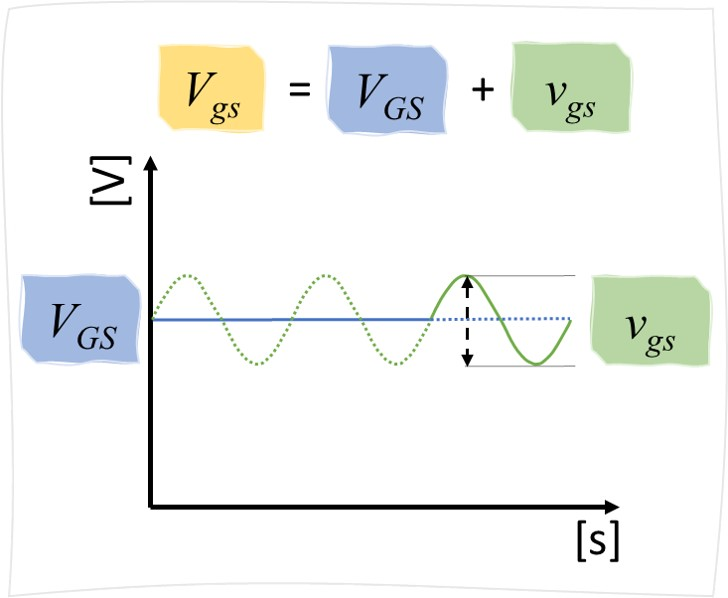
\includegraphics[scale=0.5]{./imgs/NOTATIONR00.jpg}
	\caption{Examples of the employed notation in this work.}
	\label{fig:NOTATIONR00}
\end{figure*}

\section{Analysis of an RC channel} % Unnumbered section

\subsection{Transfer function}

Consider the circuit

\begin{file}[\itshape Netlist of an RC circuit]
	
.SUBCKT RCchannel vin vout 	\newline
R1 vin vout R				\newline
C1 vout gnd! C				\newline
.ENDS
\end{file}

At node vout(s):

\centerline{$ v_{out}(s) = i(s) \cdot 1/(s \cdot C)
	$}
\vspace{\baselineskip}

\centerline{$ v_{in}(s) - v_{out}(s) = i(s) \cdot R
	$}
\vspace{\baselineskip}

\centerline{$ v_{in}(s) - i(s) \cdot 1/(s \cdot C) = i(s) \cdot R
	$}
\vspace{\baselineskip}

\centerline{$ v_{in}(s) = i(s) \cdot (R + 1/(s \cdot C))
	$}
\vspace{\baselineskip}

Thus

\centerline{$ \frac{v_{out}(s)}{v_{in}(s)} = H(s) = \frac{i(s) \cdot 1/(s \cdot C)}{i(s) \cdot (R + 1/(s \cdot C))}
	$}
\vspace{\baselineskip}

\begin{question}[\itshape Transfer function for an RC circuit]
\centerline{$ H(s) = \frac{\omega_{a}}{s + \omega_{a}}
	$}
\end{question}

Where $\tau = R \cdot C $ and $\omega_{a} = 1/ \tau$.

\subsection{Impulse response}

Applying the inverse Laplace transform in the transfer function, it is obtained:

\begin{question}[\itshape Impulse response for an RC circuit]
\centerline{$ h(t) = \omega_{a} \cdot \exp(-t * \omega_{a})
	$}
\end{question}

for t > 0.

\subsection{Magnitude of the transfer function}

\centerline{$ |H(s)| = |\frac{\omega_{a}}{s + \omega_{a}}|
	$}
\vspace{\baselineskip}

\begin{question}[\itshape Magnitude of H(s)]
\centerline{$ |H(s)| = \frac{\omega_{a}}{\sqrt{w^2 + \omega_{a}^2}}
	$}
\end{question}

\subsection{Phase of the transfer function}

\centerline{$ \theta(w) = \arctan{(\frac{\Im{H(w)}}{\Re{H(w)}})}
	$}
\vspace{\baselineskip}

\centerline{$ H(w) = \frac{\omega_{a}}{i\cdot \omega + \omega_{a}} = \frac{\omega_{a} \cdot (-i \cdot \omega + \omega_{a})}{(i \cdot \omega + \omega_{a}) \cdot (-i \cdot \omega + \omega_{a})}
	$}
\vspace{\baselineskip}

\centerline{$ H(w) = \frac{\omega_{a}^2 - i \cdot \omega \cdot \omega_{a}}{\omega^2 + \omega_{a}^2}
	$}
\vspace{\baselineskip}

\centerline{$ \Re{H(w)} = \frac{\omega_{a}^2}{\omega^2 + \omega_{a}^2}
	$}
\vspace{\baselineskip}

\centerline{$ \Im{H(w)} = \frac{-\omega \cdot \omega_{a}}{\omega^2 + \omega_{a}^2}
	$}
\vspace{\baselineskip}

\begin{question}[\itshape Phase of H(w)]
\centerline{$ \theta(w) = \arctan{(- \omega / \omega_{a})}
	$}
\end{question}

\subsection{Quantization of the model}

Considering that $\omega_{a} = \omega_{d} / FS$, where FS is the sampling frequency, the quantized model is:

\begin{question}[\itshape Transfer function for an RC circuit]
	\centerline{$ H[m] = \frac{\omega_{d} / FS}{s + \omega_{d} / FS}
		$}
\end{question}
Where m is a discrete frequency vector.

\begin{question}[\itshape Impulse response for an RC circuit]
	\centerline{$ h[n] = (\omega_{d} / FS) \cdot \exp(-n * (\omega_{d} / FS))
		$}
\end{question}
Where n is a discrete time vector.

\begin{question}[\itshape Magnitude of H(w)]
	\centerline{$ |H[m]| = \frac{\omega_{d} / FS}{\sqrt{w^2 + (\omega_{d} / FS)^2}}
		$}
\end{question}

\begin{question}[\itshape Phase of H(w)]
	\centerline{$ \theta[m] = \arctan{(- \omega /(\omega_{d} / FS))}
		$}
\end{question}

\section{Analysis of a constant time linear equalizer}

\subsection{Transfer function}

Consider the circuit

\begin{file}[\itshape Netlist of a CTLE]

.SUBCKT CTLE vinp vinn voutp voutn gnd! \newline
R1 gnd! voutp RD						\newline
M1 voutp vinp vs1 0 M1					\newline
I1 vs1 gnd! I1							\newline
R2 gnd! voutn RD						\newline
M2 voutn vinn vs2 0 M2					\newline
I2 vs2 gnd! I1							\newline
R3 vs1 vs2 RS							\newline
C1 vs1 vs2 CS							\newline
.ENDS
\end{file}

Its transfer function is:

\begin{question}[\itshape Transfer function for a CTLE circuit]
	\centerline{$ H(s) = \frac{-g_m \cdot R_D \cdot (s + \omega_a)}{(s + \omega_a \cdot (\tau + h))}
		$}
\end{question}

Where $\tau = RS \cdot CS$, $\omega_a = 1/\tau$, and $h = g_m \cdot RS / 2$.

\subsection{Impulse response}

\begin{question}[\itshape Transfer function for a CTLE circuit]
	\centerline{$ h(t) = -g_m \cdot R_D \cdot \omega_a \cdot (1 - h - \tau) \cdot exp(-t \cdot \omega_a \cdot (h + \tau) )
		$}
\end{question}

For t > 0.

\subsection{Magnitude of the transfer function}

\centerline{$ |H(w)| = \frac{g_m \cdot R_D \cdot \sqrt{w_a^2 + w^2}}{\sqrt{(w_a \cdot (\tau + h))^2 + \omega^2}}
	$}
\vspace{\baselineskip}

\subsection{Phase of the transfer function}

\centerline{$ \Re{H(w)} = \frac{g_m \cdot R_D \cdot (\omega^2 + \omega_a^2 \cdot (\tau + h))}{\omega^2 + \omega_a^2 \cdot (\tau + h)^2}
	$}
\vspace{\baselineskip}

\centerline{$ \Im{H(w)} = \frac{gm \cdot R_D \cdot \omega \cdot \omega_a \cdot (\tau + h - 1)}{\omega^2 + \omega_a^2 \cdot (\tau + h)}
	$}
\vspace{\baselineskip}

\begin{question}[\itshape Phase of H(w)]
	\centerline{$ \theta(w) = \arctan{\frac{\omega \cdot \omega_a \cdot (\tau + h - 1)}{\omega^2 + \omega_a^2 \cdot (\tau + h)^2}}
		$}
\end{question}

\subsection{Quantization of the model}

Considering that $\omega_{a} = \omega_{d} / FS$, where FS is the sampling frequency, the quantized model is:

\begin{question}[\itshape Transfer function for a CTLE circuit]
	\centerline{$ H[m] = \frac{-g_m \cdot R_D \cdot (s + (\omega_d / FS))}{(s + (\omega_d / FS) \cdot (\tau + h))}
		$}
\end{question}

\begin{question}[\itshape Transfer function for a CTLE circuit]
	\centerline{$ h[n] = -g_m \cdot R_D \cdot (\omega_d / FS) \cdot (1 - h - \tau) \cdot exp(-n \cdot (\omega_d / FS) \cdot (h + \tau) )
		$}
\end{question}

\begin{question}[\itshape Magnitude of H(w)]
\centerline{$ |H[m]| = \frac{g_m \cdot R_D \cdot \sqrt{(\omega_d / FS)^2 + \omega^2}}{\sqrt{((\omega_d / FS) \cdot (\tau + h))^2 + \omega^2}}
	$}
\vspace{\baselineskip}
\end{question}

\begin{question}[\itshape Phase of H(w)]
	\centerline{$ \theta[m] = \arctan{\frac{\omega \cdot (\omega_d / FS) \cdot (\tau + h - 1)}{\omega^2 + (\omega_d / FS)^2 \cdot (\tau + h)^2}}
	$}
\end{question}

\section{Example code}

An example code for such study can be found at: https://github.com/faverosantos/SerDes

%----------------------------------------------------------------------------------------

% References
\begin{thebibliography}{9}
	%\bibitem{techgurukula} 
	%\url{https://www.youtube.com/watch?v=bSlPaSw8pDw}
	
	%\bibitem{pornpromlikit}
	%file:///D:/Doutorado/2019\_Qualificação/Papers/Pornpromlikit\_2010.pdf
	
	%\bibitem{taylor} 
	%\url{https://math.libretexts.org/Bookshelves/Calculus/Supplemental_Modules_(Calculus)/Multivariable_Calculus/3\%3A_Topics_in_Partial_Derivatives/Taylor__Polynomials_of_Functions_of_Two_Variables}
	
	%\bibitem{sedra} 
	%Sedra, A. S. and Smith, K. C in "Microelectronics" 4th edition.	
\end{thebibliography}
%----------------------------------------------------------------------------------------

\end{document}
